\documentclass[11pt]{report}
% Same style as 1-foundations/theory/preamble.tex (the course's own documents).

\usepackage[a4paper,margin=2.3cm,headheight=14pt]{geometry}
\usepackage[T1]{fontenc}
\usepackage[utf8]{inputenc}
\usepackage{lmodern}
\usepackage{microtype}
\usepackage{booktabs}
\usepackage{longtable}
\usepackage{array}
\usepackage{xcolor}
\usepackage{enumitem}
\usepackage{amssymb}
\usepackage{amsmath}
\usepackage{fancyhdr}
\usepackage{listings}
\usepackage{tikz}
\usetikzlibrary{arrows.meta,positioning,calc,fit,shapes.geometric,decorations.pathreplacing}
\usepackage[hidelinks]{hyperref}

\definecolor{warnbg}{RGB}{255,247,230}
\definecolor{warnrule}{RGB}{204,136,0}
\definecolor{newbg}{RGB}{235,245,255}
\definecolor{newrule}{RGB}{40,110,190}
\definecolor{keybg}{RGB}{237,247,237}
\definecolor{keyrule}{RGB}{50,120,60}
\definecolor{headgray}{RGB}{90,90,90}
\definecolor{codebg}{RGB}{248,248,248}

\usepackage[most]{tcolorbox}

\newtcolorbox{warnbox}[1][]{colback=warnbg,colframe=warnrule,boxrule=0.8pt,
  left=6pt,right=6pt,top=5pt,bottom=5pt,arc=1pt,#1}
\newtcolorbox{infobox}[1][]{colback=newbg,colframe=newrule,boxrule=0.8pt,
  left=6pt,right=6pt,top=5pt,bottom=5pt,arc=1pt,#1}
% "In SWEB": where the idea shows up in the course's kernel
\newtcolorbox{swebbox}[1][]{colback=newbg,colframe=newrule,boxrule=0.8pt,
  left=6pt,right=6pt,top=5pt,bottom=5pt,arc=1pt,
  title={In SWEB},fonttitle=\bfseries\small,coltitle=white,colbacktitle=newrule,#1}
% end-of-chapter summary
\newtcolorbox{keybox}[1][]{colback=keybg,colframe=keyrule,boxrule=0.8pt,
  left=6pt,right=6pt,top=5pt,bottom=5pt,arc=1pt,
  title={Key points},fonttitle=\bfseries\small,coltitle=white,colbacktitle=keyrule,#1}

\newcommand{\tbd}{\textcolor{warnrule}{\textbf{[confirm]}}}
\newcommand{\code}[1]{\texttt{#1}}
\newcommand{\file}[1]{\texttt{\small #1}}
\newcommand{\module}[1]{\textsf{module~#1}}

\setlist[itemize]{topsep=2pt,itemsep=1.5pt,parsep=0pt,leftmargin=1.3em}
\setlist[enumerate]{topsep=2pt,itemsep=1.5pt,parsep=0pt,leftmargin=1.6em}
\setlist[description]{topsep=2pt,itemsep=1.5pt,parsep=0pt,leftmargin=1.3em}

\newcolumntype{L}[1]{>{\raggedright\arraybackslash}p{#1}}

\lstset{
  language=C,
  basicstyle=\ttfamily\small,
  keywordstyle=\color{newrule}\bfseries,
  commentstyle=\color{headgray}\itshape,
  stringstyle=\color{warnrule!80!black},
  backgroundcolor=\color{codebg},
  frame=single, rulecolor=\color{black!15}, framesep=3pt,
  xleftmargin=4pt, xrightmargin=4pt, aboveskip=6pt, belowskip=4pt,
  columns=fullflexible, keepspaces=true, showstringspaces=false,
  upquote=true, tabsize=2,
  morekeywords={size_t,ssize_t,pid_t,pthread_t,pthread_mutex_t,pthread_cond_t,
                sem_t,uint8_t,uint32_t,uint64_t,bool,_Atomic,atomic_int,
                atomic_flag,__thread,_Noreturn,__asm__,volatile,pointer,uint64}
}
\lstdefinestyle{shell}{language=bash,morekeywords={},keywordstyle=\color{black}}
\lstdefinestyle{cpp}{language=C++}

\pagestyle{fancy}
\fancyhf{}
\renewcommand{\headrulewidth}{0.4pt}
\fancyhead[L]{\small\textcolor{headgray}{SWEB interview guide}}
\fancyhead[R]{\small\textcolor{headgray}{\leftmark}}
\fancyfoot[C]{\small\thepage}
\renewcommand{\chaptermark}[1]{\markboth{\thechapter\ \ #1}{}}
\fancypagestyle{plain}{\fancyhf{}\renewcommand{\headrulewidth}{0pt}\fancyfoot[C]{\small\thepage}}

\renewcommand{\arraystretch}{1.25}
\setlength{\parskip}{3pt}
\setlength{\parindent}{0pt}
\setlength{\emergencystretch}{3em}   % fewer overfull lines with long \code words

% guide additions
\newtcolorbox{lockbox}[1][]{colback=warnbg,colframe=warnrule,boxrule=0.8pt,
  left=6pt,right=6pt,top=5pt,bottom=5pt,arc=1pt,
  title={Locking},fonttitle=\bfseries\small,coltitle=white,colbacktitle=warnrule,#1}
\newtcolorbox{trapbox}[1][]{colback=warnbg,colframe=warnrule,boxrule=0.8pt,
  left=6pt,right=6pt,top=5pt,bottom=5pt,arc=1pt,
  title={Trap},fonttitle=\bfseries\small,coltitle=white,colbacktitle=warnrule,#1}
\lstset{morekeywords={ScopeLock,Mutex,Condition,SpinLock,ArchThreadRegisters,ArchMemoryMapping},
  breaklines=true, breakatwhitespace=true, postbreak=\mbox{\textcolor{headgray}{$\hookrightarrow$}\space}}
\renewcommand{\file}[1]{\texttt{#1}}   % inherit the size of the surrounding text (tables use \footnotesize)

\fancyhead[L]{\small\textcolor{headgray}{A1-10 shared page -- the bare minimum}}
\fancyhead[R]{}
\newcommand{\step}[2]{\par\medskip\noindent{\large\bfseries #1}\hfill{\file{#2}}\par\nopagebreak\smallskip}

\begin{document}

{\centering {\LARGE\bfseries A1-10 shared page -- the bare minimum\par}\vspace{6pt}}

\begin{infobox}
Only what you need to make it work. Every line explained: \file{walkthrough.pdf} in this folder.
Start: \code{task start a1-10}. Done: \code{task test} shows \textbf{9 of 9}.
\end{infobox}

\section*{The idea in 3 sentences}

\begin{enumerate}
  \item \code{shm\_attach(7)} in two processes puts the \textbf{same physical page} into both -- what one
        writes, the other reads.
  \item The kernel keeps \textbf{one small table}: for each key (1--15) the physical page and \textbf{how many
        processes} use it.
  \item The page is only freed when that count drops to \textbf{0} -- so unmapping it must \textbf{not}
        free it.
\end{enumerate}

\begin{center}
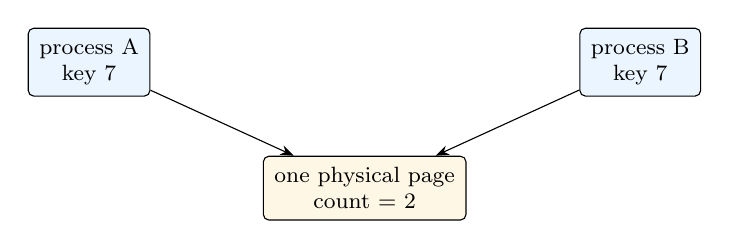
\begin{tikzpicture}[font=\footnotesize, box/.style={draw,rounded corners=2pt,align=center,inner sep=4pt}]
  \node[box,fill=newbg] (a) at (0,0) {process A\\key 7};
  \node[box,fill=newbg] (b) at (7,0) {process B\\key 7};
  \node[box,fill=warnbg] (p) at (3.5,-1.6) {one physical page\\count = 2};
  \draw[-{Stealth}] (a) -- (p); \draw[-{Stealth}] (b) -- (p);
\end{tikzpicture}
\end{center}

\section*{Checklist -- 6 places}

\begin{tabular}{@{}l L{6.2cm} L{7.4cm}@{}}
\toprule
\# & What & File\\\midrule
1 & numbers, libc, \code{case}s (plumbing) & \file{syscall-definitions.h}, \file{nonstd.h/.c}, \file{Syscall.cpp}\\
2 & unmap \emph{without} freeing & \file{ArchMemory.h/.cpp}\\
3 & the table (new class) & new \file{common/include/mm/SharedPages.h} + \file{common/source/mm/SharedPages.cpp}\\
4 & create the table at boot & \file{common/source/kernel/main.cpp}\\
5 & attach + detach & \file{UserProcess.h/.cpp}\\
6 & clean up when a process ends & \file{UserProcess.cpp} (destructor)\\
\bottomrule
\end{tabular}

% =====================================================================================
\step{1 -- Plumbing}{syscall-definitions.h · nonstd.h · nonstd.c · Syscall.cpp}

\begin{lstlisting}[style=cpp]
// syscall-definitions.h
#define sc_shm_attach 1680
#define sc_shm_detach 1681

// nonstd.h  (needs #include "types.h" at the top)
extern void* shm_attach(size_t key);
extern int shm_detach(size_t key);

// nonstd.c
void* shm_attach(size_t key) { return (void*) __syscall(sc_shm_attach, key, 0, 0, 0, 0); }
int shm_detach(size_t key)   { return __syscall(sc_shm_detach, key, 0, 0, 0, 0); }

// Syscall.cpp, in the switch
case sc_shm_attach: return_value = currentThread->getProcess()->shmAttach(arg1); break;
case sc_shm_detach: return_value = currentThread->getProcess()->shmDetach(arg1); break;
\end{lstlisting}

% =====================================================================================
\step{2 -- Unmap without freeing}{ArchMemory.h · ArchMemory.cpp}

\begin{lstlisting}[style=cpp]
// ArchMemory.h - add a parameter with a default (old calls keep working)
bool unmapPage(uint64 virtual_page, bool free_physical_page = true);

// ArchMemory.cpp - first line of unmapPage, and wrap the freePPN line in an if
bool ArchMemory::unmapPage(uint64 virtual_page, bool free_physical_page)
  ...
  if (free_physical_page)
    PageManager::instance()->freePPN(m.page_ppn);
\end{lstlisting}
\textbf{Why:} a shared page still belongs to the other process.

% =====================================================================================
\step{3 -- The table}{new files SharedPages.h / SharedPages.cpp in mm/}

\begin{lstlisting}[style=cpp]
// common/include/mm/SharedPages.h
#pragma once
#include "types.h"
class Mutex;
#define SHM_MAX_KEYS 16
#define SHM_BASE 0x0000400000000000ULL      // key k lives at SHM_BASE + k pages

class SharedPages
{
  public:
    static SharedPages* instance();
    static void init();
    size_t acquire(size_t key);              // count + 1 (creates the page), returns the ppn
    void release(size_t key);                // count - 1 (frees the page at 0)
  private:
    SharedPages();
    static SharedPages* instance_;
    struct Entry { size_t ppn; size_t references; };
    Mutex* lock_;
    Entry entries_[SHM_MAX_KEYS];
};
\end{lstlisting}

\begin{lstlisting}[style=cpp]
// common/source/mm/SharedPages.cpp
#include "SharedPages.h"
#include "PageManager.h"
#include "Mutex.h"
#include "ScopeLock.h"
#include "assert.h"

SharedPages* SharedPages::instance_ = nullptr;
void SharedPages::init() { instance_ = new SharedPages(); }
SharedPages* SharedPages::instance() { return instance_; }

SharedPages::SharedPages() : lock_(new Mutex("SharedPages::lock_"))
{
  for (Entry& entry : entries_) { entry.ppn = 0; entry.references = 0; }
}

size_t SharedPages::acquire(size_t key)
{
  ScopeLock lock(*lock_);
  if (entries_[key].ppn == 0)
    entries_[key].ppn = PageManager::instance()->allocPPN();   // new, zeroed page
  entries_[key].references++;
  return entries_[key].ppn;
}

void SharedPages::release(size_t key)
{
  ScopeLock lock(*lock_);
  entries_[key].references--;
  if (entries_[key].references == 0)
  {
    PageManager::instance()->freePPN(entries_[key].ppn);       // last user gone
    entries_[key].ppn = 0;
  }
}
\end{lstlisting}

% =====================================================================================
\step{4 -- Create the table at boot}{main.cpp}

\begin{lstlisting}[style=cpp]
#include "SharedPages.h"          // at the top
...
Scheduler::instance();
SharedPages::init();               // new line, in startup()
\end{lstlisting}
\textbf{Why:} SWEB does not run constructors of global objects.

% =====================================================================================
\step{5 -- Attach and detach}{UserProcess.h · UserProcess.cpp}

\begin{lstlisting}[style=cpp]
// UserProcess.h - public:
size_t shmAttach(size_t key);
size_t shmDetach(size_t key);
// UserProcess.h - private, at the bottom:
bool shm_attached_[16] = {};               // which keys this process has mapped
\end{lstlisting}

\begin{lstlisting}[style=cpp]
// UserProcess.cpp - #include "SharedPages.h" and "ScopeLock.h" at the top
size_t UserProcess::shmAttach(size_t key)
{
  if (key == 0 || key >= SHM_MAX_KEYS)
    return 0;
  size_t vpn = SHM_BASE / PAGE_SIZE + key;
  size_t ppn = SharedPages::instance()->acquire(key);     // 1. count + 1
  bool already;
  {
    ScopeLock lock(thread_lock_);                         // 2. then map (other lock)
    already = shm_attached_[key];
    if (!already)
    {
      bool mapped = arch_memory_->mapPage(vpn, ppn, 1);
      assert(mapped);
      shm_attached_[key] = true;
    }
  }
  if (already)
    SharedPages::instance()->release(key);                // counted twice: undo
  return vpn * PAGE_SIZE;
}

size_t UserProcess::shmDetach(size_t key)
{
  if (key == 0 || key >= SHM_MAX_KEYS)
    return (size_t) -1;
  {
    ScopeLock lock(thread_lock_);                         // 1. unmap, keep the page
    if (!shm_attached_[key])
      return (size_t) -1;
    arch_memory_->unmapPage(SHM_BASE / PAGE_SIZE + key, false);
    ArchMemory::flushTlb();
    shm_attached_[key] = false;
  }
  SharedPages::instance()->release(key);                  // 2. count - 1
  return 0;
}
\end{lstlisting}

% =====================================================================================
\step{6 -- Clean up when a process ends}{UserProcess.cpp, \textasciitilde UserProcess}

Between \code{delete loader\_;} and \code{delete arch\_memory\_;}:
\begin{lstlisting}[style=cpp]
for (size_t key = 1; key < SHM_MAX_KEYS; ++key)
{
  if (shm_attached_[key])
  {
    arch_memory_->unmapPage(SHM_BASE / PAGE_SIZE + key, false);
    SharedPages::instance()->release(key);
  }
}
\end{lstlisting}
\textbf{Why:} \code{delete arch\_memory\_} frees every mapped page -- also the shared one, if a process
ends without detaching.

\begin{keybox}[title={The three rules to remember}]
\begin{enumerate}
  \item Count the users; free only at 0.
  \item Unmapping a shared page never frees it (\code{false}).
  \item Never hold both locks: attach = count, then map; detach = unmap, then count.
\end{enumerate}
\end{keybox}

\end{document}
